%!TEX root = ../Bachelorseminar-RoboticSwarms.tex
\begin{figure*}
  \centering
  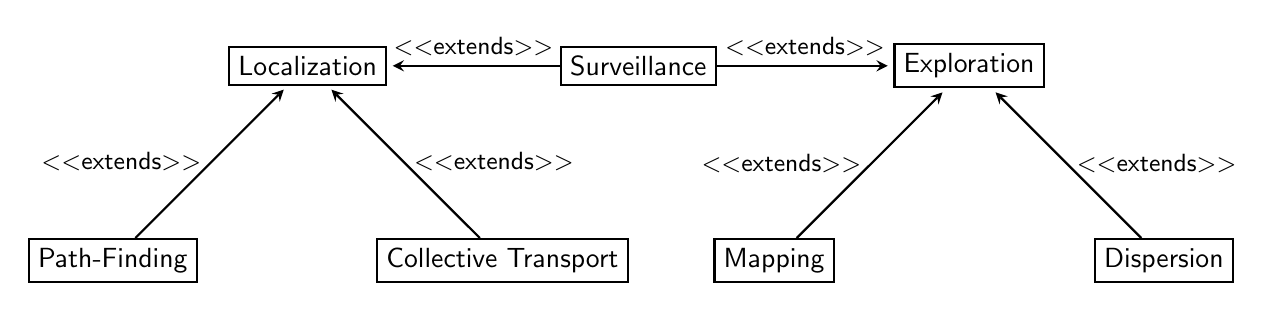
\begin{tikzpicture}[->,>=stealth,shorten >=2pt,auto,node distance=3.5cm,
    thick,main node/.style={fill=white,draw,font=\sffamily}]
    \node[main node] (1) {Localization};
    \node[main node] (2) [below left of=1] {Path-Finding};
    \node[main node] (3) [below right of=1] {Collective Transport};
    \node[main node] (4) [right of=1,node distance=4.2cm] {Surveillance};
    \node[main node] (5) [right of=4,node distance=4.2cm] {Exploration};
    \node[main node] (7) [below left of=5] {Mapping};
    \node[main node] (6) [below right of=5] {Dispersion};

    \path[every node/.style={font=\sffamily\small}]
      (2) edge node [left] {$<<$extends$>>$} (1)
      (3) edge [right] node[right] {$<<$extends$>>$} (1)
      (4) edge [right] node[above] {$<<$extends$>>$} (1)
      (4) edge [right] node[above] {$<<$extends$>>$} (5)
      (6) edge [right] node[right] {$<<$extends$>>$} (5)
      (7) edge [right] node[left] {$<<$extends$>>$} (5);
  \end{tikzpicture}
  \caption{Technique Hierarchy Overview} \label{fig:TechniquesMindMap}
\end{figure*}

After pointing out some applications implementing important techniques used in robotic swarms, we will now provide an in-depth study for these techniques. For every technique, we will make comparisons between different algorithms used by a technique, the problems that are solved and the the problems that are yet to be solved. This chapter thus serves to provide a good overview of ways to implement a technique. 
    \subsection{Exploration}
    %!TEX root = ../../Bachelorseminar-RoboticSwarms.tex

\subsubsection{Collaborative multi-robot exploration [1]}
\cite{burgard2005coordinated}

    \subsection{Mapping}
    %!TEX root = ../../Bachelorseminar-RoboticSwarms.tex

    \subsection{Dispersion}
    %!TEX root = ../../Bachelorseminar-RoboticSwarms.tex

One of the key techniques used in robotic swarms is dispersion. The goal of dispersion in the context of robotic swarms is to scatter the individual robots in an environment such that every section of the environment can be covered. In this section we will focus on non-location oriented algorithms. If prior knowledge about the exact location is provided, a formation technique should be used.

\subsubsection{Algorithms}
	The following dispersion algorithms are the most widely used algorithms and thus will be taken into our analysis. A very brief description is given of each algorithm. For more information on the operation of these algorithms, please consult the references.\\

	\textbf{Location-Free Dispersion Algorithms}
	\begin{itemize}
		\item \textbf{Depth-First Leader-Follower Strategy (\emph{DFLF})}\cite{hsiang2004algorithms}:\\
			A \emph{Depth First Search}(DFS) inspired algorithm in which the swarm has one leader at any given point in time. The robotic swarm has the overview of a map in which specific regions, called \emph{pixels}, are defined. \emph{Frontier pixels}, are pixels which haven't been traversed yet. The leader robot keeps looking for frontier pixels until there are none left and stops and tells its \emph{successor robot} to be the leader. If there are no successors left, the algorithm halts and the total dispersion of the area. The other robots always try to follow the leader and traverse the tiles around it.
		\item \textbf{Breadth-First Leader-Follower (\emph{BFLF})}\cite{hsiang2004algorithms}:\\
			A \emph{Breadth First Search}(\emph{BFS}) inspired algorithm, which does not exactly perform \emph{BFS}, but approximates it. It is a more complex algorithm than the \emph{DFLF} algorithm, but has to make fewer moves to fully cover the map. In an extension of the \emph{DFLF} algorithm, the \emph{BFLF} algorithm also contains a waiting state, in which a robot pauses to make the next move. Furthermore, instead of having only one leader, this algorithm allows for multiple leaders. The leaders again strive to find all the frontier pixels, but now also make sure that the follower robots don't stray to far away. Once no frontier pixels can be found by the leader, the leader waits for the followers to arrive and passes on its leadership to one of the followers, the successor. The \emph{BFLF} strategy tries to create as many paths as possible. Visited pixels form a tree, the tree can be branched, which then represent the alternate pixels reachable from that pixel. This branching balances the flow by giving the possiblity to go through pixels multiple times, to be able to go into differerent directions.
	\end{itemize}
	\textbf{Range-Based Dispersion Algorithms}
	\begin{itemize}
		\item \textbf{Directed Dispersion/Disperse Uniformly}\cite{mclurkin2007distributed}:\\
			The directed dispersion algorithm has the goal to disperse the robots quickly and uniformly, while keeping the robots connected. The algorithm consists of two sub-algorithms: \emph{disperseUniformly} and \emph{frontierGuidedDispersion}. The \emph{disperseUniformly} algorithm spreads the robots evenly with given constraints. It works by calculating an opposite direction vector of the positions of the nearest robots. This means that communication between robots is of vital importance. The \emph{frontierGuidedDispersion} directs robots towards unexplored areas, while keeping the robots connected. It uses robots which are on the frontiers of explored space to guide the Swarm in unexplored space. An optimal path is created for the other robots to move optimally towards the frontier. For an exact description of the implementation of these algorithms please see \cite{mclurkin2007distributed}.
		\item \textbf{Random Walk}\cite{morlok2007dispersing}:\\
			This algorithm has 2 states: \emph{walking} and \emph{avoid obstacle}. In the \emph{walking} state each robot keeps going straight with an orientation which randomizes over a certain time interval until there is an object and switches to the \emph{avoid obstacle} state. In the case that it detects a possible collision, the robot changes orientation dramatically until the obstacle has been avoided and continues in the \emph{walking} state.
		\item \textbf{Follow Wall}\cite{morlok2007dispersing}:\\
			The follow wall algorithm has 4 states: \emph{find wall}, \emph{align to wall}, \emph{follow wall} and \emph{navigate corner}. The details of this algorithm will not be discussed, as there are quite a few major flaws in this algorithm. This algorithm does not take the existance of other robots into account and thus it is possible for robots to see each other as walls. The usage of this algorithm for dispersion is thus very limited and should be avoided.
		\item \textbf{Seek Open}\cite{morlok2007dispersing}:\\
			By calculating an average obstacle vector with support of distance censors, a vector in the exact opposite direction is calculated and the robot, will follow this vector. Depending on the magnitede of the vector, a new assesment will be done once the robot reaches the approximated location. This means that the robot does not need to take further care of collisions with walls, but it is possible for robots to run into each other, or other dynamically moving objects, unless collision avoindance is separetely implemented.
		\item \textbf{Fiducial} \cite{morlok2007dispersing}:\\
			By using a beacon system, every robot is able to get the relative location of other robots within a certain range. This information is the used to steer away from the other robots. If no robots are in range, the robot uses the \emph{Random Walk} algorithm.
		\item \textbf{Clique-Intensity}\cite{ludwig2006robotic}:\\
			This algorithm uses the connectivity in a cyclic graph for swarm robots to disperse the robots, by knowing their relative distance. By using multiple behaviours as many robots as possible try to stay connected to only one other robot, thus making a very spread out system, which still remains connected.
	\end{itemize}

  \begin{table}[H]
  \renewcommand{\arraystretch}{1.3}
  \label{table_alg_dispersion}
  \centering
    \begin{tabular}{|l|p{2.2cm}|p{2.2cm}|p{2.2cm}|}
    \hline
    \bfseries Algorithm & \bfseries Type & \bfseries Performance & \bfseries Scalability\\
    \hline
    \bfseries DFLF& Location-Free & Medium-High & High\\\hline
    \bfseries BFLF & Location-Free & High & High\\\hline
    \bfseries Directed Dispersion & Range-Based & Medium & High\\\hline
    \bfseries Random Walk& Range-Based & Low & Low\\\hline
    \bfseries Follow Wall& Range-Based & Low & Low\\\hline
    \bfseries Seek Open& Range-Based & Low & Medium\\\hline
    \bfseries Fiducial& Range-Based & Medium & High\\\hline
    \bfseries Clique-Intensity& Range-Based & High & High\\\hline
    \end{tabular}
  \caption{Overview of Common Dispersion Algorithms}
  \end{table}

  \subsubsection{Problems}
  \textbf{Range-Based}

  Starting from the simpler Algorithms such as random walk and wall following, we show the problems that the dispersion technique has faced in the past and how the newer algorithms have solved these problems. The \emph{Random Walk} algorithm has to be one of the simpelest algorithms, the problem this algorithm faces though, is that dispersiveness of the robots does not guarantee uniform dispersion. The algorithm can be seen as a brute-force approach, it possibly achieves our end-goal, but it does not do this in an optimal and scalable way.

  \emph{Wall Following} is an algorithm which is used a lot in robotic swarms, however it is not very effective by itself and faces many problems with scalability.  One of the main problems with scalability is the fact that the robot does not distinguish other robots and actual walls. This causes an extereme amount of collisions and thus with large amounts of robots, this algorithm becomes near to useless. 

  The \emph{Seek Open} algorithm is a good example of the real usage of Range-Based navigation, due to the fact that it actually uses the magnitudes of the data provided and does calculations in order to find the best position to move towards. The problem that this algorithm faces however is that it should be implemented with a collision avoidance algorithm. The algorithm is not really adapted to work with other dynamic objects, such as other robots. It is therefore not a very scalable algorithm by itself.

  The \emph{Fiducial} algorithm uses the Random Walk algorithm. A problem with the Random Walk algorithm has been solved here: the beacon like system, prevents the robots from running into each other. The Fiducial algorithm does not have any specific problems, however it still is a brute-force approach and thus does not guarantee uniform dispersion.

  The main problem with the \emph{Clique-Intensity} algorithm is the fact that due to high amounts of noise in the wireless intensity signals there is a lot of uncertainty in some real world applications. In a perfect situation, the algorithm would also work near perfectly. The work in this area has mostly been theoretical, real-world application is very different compared to theoretical situations.\\

  \textbf{Location-Free}
  The \emph{BFLF} algorithm, requires the robots to travel less compared to the \emph{DFLF} algortihm. The DFLF algorithm is furthermore also more computationally expensive than the DFLF algorithm. There is no big difference further during the execution of both algorithms, and thus BFLF has the preference. The problems that these types of algorithms face are not theoretical, but are coming forth from the category that they're in: often it is impossible to know the exact location, even if it's relative. There are quite a few ways that people try to achieve to create a relative position grid, however it difficult if not impossible to achieve in many real world applications.\\

\subsubsection{Remaining-Problems}
  The remaining problems in dispersion algorithms can be generally categorized into range-based problems and location-free problems, since all of the algorithms that are in these categories, are facing similar problems.
  The focus needed for the range-based approach needs to be on the uniformity of the dispersion. So how can we guarantee uniformity when dispersing the robots.
  The focus needed for location-free approaches is: how do we actually implement this in real world applications. There are minor to no problems in theory, however to actually bring the relative positioning into a grid is quite difficult. Research in this area should be focussed on how to create these relative positioning grids into a dependable and accurate manner.

    \subsection{Localization}
    %!TEX root = ../../Bachelorseminar-RoboticSwarms.tex

    \subsection{Path-finding}
    %!TEX root = ../../Bachelorseminar-RoboticSwarms.tex

    \subsection{CollectiveTransport}
    %!TEX root = ../../Bachelorseminar-RoboticSwarms.tex

    \subsection{Surveillance}
    %!TEX root = ../../Bachelorseminar-RoboticSwarms.tex

Surveillance is the last technique that is going to be discussed in this paper, and for good reason. 
As can be seen in the figure \ref{fig:TechniquesMindMap}, surveillance is a technique that uses both the techniques exploration and localization.
This is obvious, because when a robotic swarm is surveilling an unknown environment, it has to explore the environment and has to localize disturbances.
So it makes sense to review this technique as last, as it references algorithms already used in other techniques.  
Surveillance as a technique is also very close to the application domain, as surveillance is more of a goal than a technique. 
But, because it combines other techniques and is used in many applications, it is deemed useful to review a few popular algorithms. 
In some surveillance algorithms, we also consider the formation technique, in which the robot swarms have to dynamically retain their formation which is important for most of the surveillance algorithms. 

\subsubsection{Surveillance Algorithms}
 \\

\textbf{Location-free surveillance}
\begin{itemize}
\item \textbf{Kinetic Theory of Gases Algorithm}\\
The first surveillance algorithm which will be expanded on is a novel one, based on the article Robotic Simulation of Gases for a Surveillance Task. \cite{Kerr2005}.
The goal that is defined for this algorithm is that it requires a swarmof robots to monitor a corridor, by sweeping through it while avoiding obstacles. 
The problem reaching this goal is maintaining spatial coverage, especially after passing obstacles, while the swarm robots are only equipped with limited sensors and communication.
The algorithm that is used is described as a Kinetic Theory algorithm, which is modelled after the movement of gases. 
In this algorithm, every molecule of a gas cloud is modeled as a robot, but because robots are not that small, this system is made for a larger scale. 
Every robot has 24 different sonar sensors to detect walls/obstacles, plus the capability to communicate with low bandwidth radio frequency communication. 
The goal direction is detected with a light sensor.\\
The algorithm works as follows. Each robots tries to detect the goal destination. If a robot finds it, it communicates this to all other to specify the direction in which they have to go. 
It is pretty similar to the flocking algorithm, but the difference in algorithms is the way they handle internal and external collisions (i.e. collisions between robots and walls). 
When collisions in the Kinetic Theory algorithm are detected, the robots calculates its new position and orientation depending on the speed and orientation of the obstacle (robot or wall). 
This is modelled after the way particles of a gas cloud move when colliding. 
	
\item \textbf{Scouts and Rangers}\\
	2000 - Rybski - A Team of Robotic Agents for Surveillance
\end{itemize}

\textbf{Location-based surveillance}
\begin{itemize}
\item \textbf{Networked Robotic Surveillance}\\
	2012 - Ghaffarkhah - Path Planning for Networked Robotic Surveillance
\item \textbf{Surveillance Event Agents}\\
	2006 - Roman-Ballesteros - A Framework for Cooperative Multi-Robot Surveillance Tasks
\end{itemize}

\textbf{Range-free surveillance}
\begin{itemize}
\item \textbf{Stochastic Strategies}\\
	2005 - Grace - stochastic Strategies for Autonomous Robotic Surveillance
\end{itemize}

\textbf{Range-based surveillance}
\begin{itemize}
\item \textbf{Dynamic Directed Movement Behaviour}\\
	2013 - Mullen - Reactive Coordination and Adaptive Lattice Formation in Mobile Robotic surveillance Swarms
\end{itemize}

  \begin{table}[!t]
  \renewcommand{\arraystretch}{1.3}
  \label{table_example}
  \centering
    \begin{tabular}{|l|p{2.2cm}|p{2.2cm}|p{2.2cm}|}
    \hline
    \bfseries Algorithm & \bfseries Type & \bfseries Performance & \bfseries Scalability\\
    \hline
    \bfseries Zooi1 & Range-free & High & High\\\hline
    \bfseries zooi2 & Range-free & Medium & Medium\\\hline
    \bfseries Zooi3 & Range-free & Low  & High\\\hline

    \end{tabular}
  \caption{Overview of Surveillance Algorithms}
  \end{table}


\subsubsection{Problems}
There are a lot of problems. Deal with it. 


\subsubsection{Remaining problems}
Yeah, a lot of them. 













